\documentclass[12pt,A4 paper]{article}
\usepackage{caption}
\usepackage{tikz}
\usepackage{refstyle}
\usepackage{graphicx}
\usepackage{graphics}
\usepackage{listings}
\usepackage{subfig}
\usepackage{float}
\graphicspath{{/storage/self/primary/Download/latex1/figs}}
\begin{document}
\title{\textbf{CIRCLE}}
\date{}
\maketitle

\begin{enumerate}
	\item In the given \figref{1},the quadrilateral $PQRS$ circumscribes a circle.Here $PA+CS$ is equal to : 

\begin{figure}[H]
	        \centering
		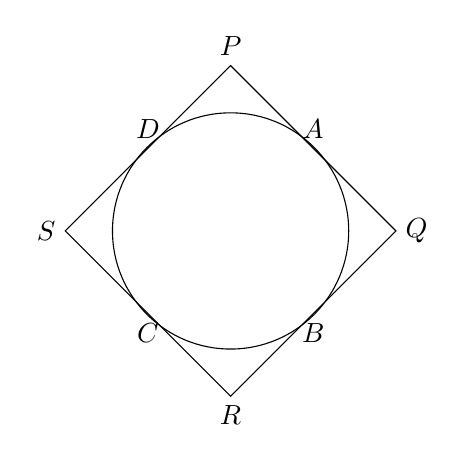
\begin{tikzpicture}
     \draw (0,0)circle(1.5cm);    
     \draw (-2.1,0)-- node[below]{$C$}(0,-2.1)--node[below]{$B$}(2.1,0)--node[above]{$A$}(0,2.1)--node[above]{$D$}cycle;
     \node[right] at (2.1,0){$Q$};    
     \node[left] at (-2.1,0){$S$};
     \node[above] at (0,2.1){$P$};
     \node[below] at (0,-2.1){$R$};    
\end{tikzpicture}

		\caption{}
		\label{fig:1}
\end{figure}



 \begin{figure}[H]
	        \centering
	         \setlength{\tabcolsep}{80pt}
 \renewcommand{\arraystretch}{2}
 
  \begin{tabular}{l c}
	  a)QR & b)PR \\
	  c)PS & d)PQ
  \end{tabular}

 \end{figure}




\item In the given \figref{2},$\vec{O}$ is the center of the circle.$AB$ and $AC$ are tangents drawn to the circle from point $\vec{ A}$.If $\angle BAC=65^{\circ}$, then find the measure of $\angle BOC$.


	\begin{center}
\begin{figure}[H]
	        \centering
	        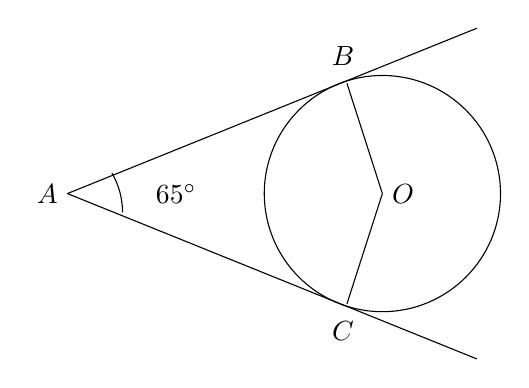
\begin{tikzpicture}

     \draw (0,0)circle(1.5cm);
     \draw(-4,0)--(1.2,2.1);
     \draw(-4,0)--(1.2,-2.1);
     \draw(0,0)--(-0.45,1.4);
     \draw(0,0)--(-0.45,-1.4);
     \draw(-3.3,-0.24)arc(0:30:1cm);
     \node[left]at(-4,0){$A$};
     \node[right]at(-3,0){$65^{\circ}$};
     \node[above]at(-0.5,1.5){$B$};
     \node[below]at(-0.5,-1.5){$C$};
     \node[right]at(0,0){$O$};
\end{tikzpicture}

		\caption{}
		\label{fig:2}
        \end{figure}
	\end{center}




\item In the given \figref{3},$\vec{ O}$ is the centre of the circle and $QPR$ is a tangent to it at$\vec{ P}$. Prove that $\angle QAP+ \angle APR$= $90^{\circ}$.
\begin{figure}[H]
	        \centering
	        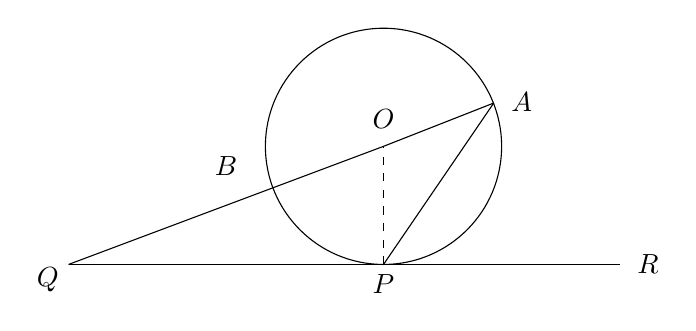
\begin{tikzpicture}
    \draw(0,0)circle(1.5cm);
    \draw(-4,-1.5)--(3,-1.5);
    \draw(-4,-1.5)--(0,0)--(1.4,0.55);
    \draw(1.4,0.55)--(0,-1.5);
    \draw[dashed](0,-1.5)--(0,0);
    \node[right]at(1.5,0.56){$A$};
    \node[left]at((-4,-1.7){$Q$};
    \node[above]at(-2,-0.5){$B$};
    \node[above]at(0,0.1){$O$};
    \node[below]at(0,-1.5){$P$};
    \node[right]at(3.1,-1.5){$R$};
\end{tikzpicture}


		\caption{}
		\label{fig:3}

        \end{figure}





\item In the given \figref{4},$PQ$ is tangent to the circle centred at $\vec{ O}$.If $\angle AOB= 95^{\circ}$, then the measure of $\angle ABQ$ will be
\begin{figure}[H]
	        \centering
	        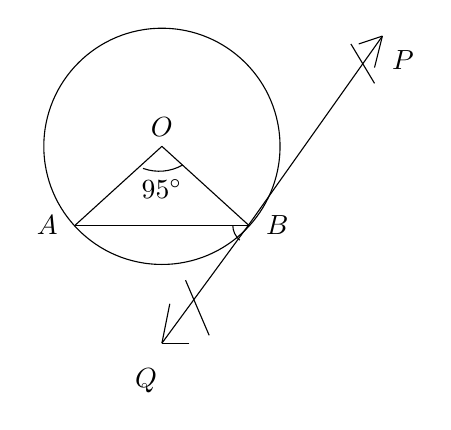
\begin{tikzpicture}
    \draw(0,0)circle(1.5cm);
    \draw(-1.1,-1)--(1.1,-1);
    \draw(-1.1,-1)--(0,0);
    \draw(1.1,-1)--(0,0);
    \draw(-0.24,-0.28)arc(250:300:0.6cm);
    \draw(0,-2.5)--(1.1,-1)--(2.8,1.4);
    \draw(2.7,1)--(2.8,1.4);
    \draw(2.8,1.4)--(2.5,1.3);
    \draw(2.4,1.3)--(2.7,0.8);
    \draw(0.1,-2)--(0,-2.5);
    \draw(0.35,-2.5)--(0,-2.5);
    \draw(0.3,-1.7)--(0.6,-2.4);
    \draw(0.9,-1)arc(180:230:0.25cm);
    \node[above]at(0,0){$O$};
    \node[left]at(-1.2,-1){$A$};
    \node[right]at(1.2,-1){$B$};
    \node[right]at(2.8,1.1){$P$};
    \node[below]at(-0.2,-2.7){$Q$};
    \node[below]at((0,-0.3){$95^{\circ}$};
   
\end{tikzpicture}


		\caption{}
		\label{fig:4}
        \end{figure}


\begin{figure}[H]
	        \centering
	        \setlength{\tabcolsep}{80pt}
 \renewcommand{\arraystretch}{2}
 
  \begin{tabular}{l c}
       A)47.5$^{\circ}$ & B)42.5$^{\circ}$ \\
       C)85$^{\circ}$& D)95$^{\circ}$
  \end{tabular}

        \end{figure}






\item
  \begin{enumerate}
	  \item Two tangents $TP$ and $TQ$ are drawn between to a circle with centre $\vec{O}$ from an external point $\vec{T}$ (\figref{5}). Prove that $\angle PTQ = 2 \angle OPQ$.
\begin{figure}[h]
	        \centering
	        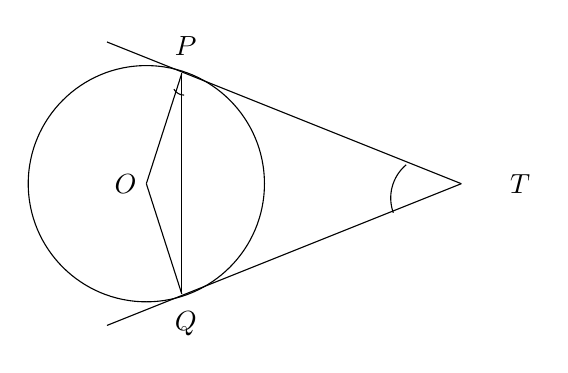
\begin{tikzpicture}

     \draw (0,0)circle(1.5cm);
     \draw(4,0)--(-0.5,1.8);
     \draw(4,0)--(-0.5,-1.8);
     \draw(0,0)--(0.45,1.4);
     \draw(0,0)--(0.45,-1.4);
     \draw(3.3,0.24)arc(130:200:0.55cm);
     \draw(0.45,1.4)--(0.45,-1.4);
     \draw(0.35,1.2)arc(210:270:0.15cm);
     \node[left]at(5,0){$T$};
     \node[above]at(0.5,1.5){$P$};
     \node[below]at(0.5,-1.5){$Q$};
     \node[left]at(0,0){$O$};
\end{tikzpicture}

		\caption{}
		\label{fig:5}
        \end{figure}






\begin{center}
    \title{OR}
\end{center}
\item In the given \figref{6},a circle is inscribed in a quadrilateral $ABCD$ in which $\angle B =90 ^{\circ}$.If $AD=17cm,AB=20cm and DS=3cm$, then find the radius of the circle.

\begin{figure}[h]
	        \centering
	        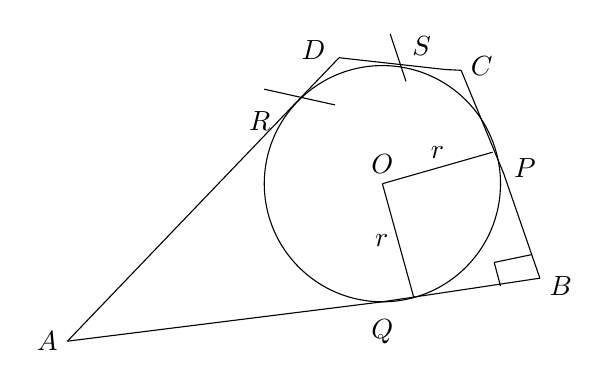
\begin{tikzpicture}

     \draw (0,0)circle(1.5cm);
     \draw(-4,-2)--(0,-1.5)--(2,-1.2);
     \draw(-4,-2)--(-0.55,1.6);
     \draw(-0.55,1.6)--(0.8,1.45)--(1,1.44);
     \draw(2,-1.2)--(1.54,0.13)--(1,1.44);
     \draw(0,0)--node[above]{$r$}(1.4,0.4);
     \draw(0,0)--node[left]{$r$}(0.4,-1.45);
     \draw(0.1,1.9)--(0.3,1.3);    
     \draw(-0.6,1)--(-1.5,1.2);
     \draw(1.42,-1)--(1.9,-0.9);
     \draw(1.42,-1)--(1.5,-1.3);
     \node[left]at(-4,-2){$A$};
     \node[below]at(0,-1.6){$Q$};
     \node[right]at(2,-1.3){$B$};
     \node[right]at(1.55,0.2){$P$};
     \node[above]at(0.5,1.5){$S$};
     \node[left]at(-1.3,0.8){$R$};
     \node[right]at(1,1.5){$C$};
     \node[left]at(-0.6,1.7){$D$};
     \node[above]at(0,0){$O$};
\end{tikzpicture}

		\caption{}
		\label{fig:6}
\end{figure}
   \end{enumerate}






\item The discus throw is an event in which an athlete attempts to throw a discus (as shown in the given \figref{0}).The athlete spins anti-clockwise around one and a half times through a circle, then releases the throw. When released, the discus travels along tangent to the circular spin orbit.


\begin{figure}[H]	

	        \centering
		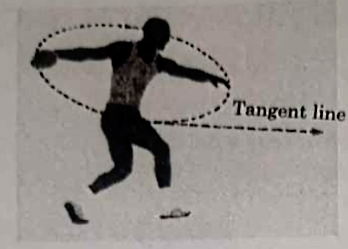
\includegraphics[width=\columnwidth]{figs/fig0.png}
		\caption{}
		\label{fig:0}
\end{figure}



In the given \figref{7}, $AB$ is one such tangent to a circle of radius 75 cm.Point $\vec{ O}$ is centre of the circle and $\angle ABO= 30^{\circ}$.$PQ$ is parallel to $OA$.



\begin{figure}[H]
	        \centering
	        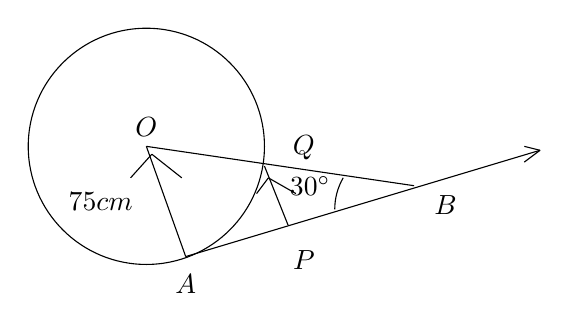
\begin{tikzpicture}
         \draw(0,0)circle(1.5cm);
         \draw(0,0)--(0.5,-1.4);
         \draw(0.5,-1.4)--(5,-0.05);
         \draw(0,0)--(3.4,-0.5);
         \draw(1.5,-0.25)--(1.8,-1);
         \draw(2.5,-0.4)arc(150:180:0.8cm);
         \draw(-0.2,-0.4)--(0.07,-0.1);
         \draw(0.07,-0.1)--(0.45,-0.4);
         \draw(1.55,-0.4)--(1.9,-0.6);
         \draw(1.55,-0.4)--(1.4,-0.6);
         \draw(4.8,0)--(5,-0.05);
         \draw(4.8,-0.2)--(5,-0.05);
         
         \node[left]at(-0.05,-0.7){$75cm$};
         \node[right]at(1.7,-0.5){$30^{\circ}$};
         \node[above]at(0,0){$O$};
         \node[below]at(0.5,-1.5){$A$};
         \node[below]at(2,-1.2){$P$};
         \node[below]at(3.8,-0.5){$B$};
         \node[above]at(2,-0.3){$Q$};
     \end{tikzpicture}

		\caption{}
		\label{fig:7}
        \end{figure}



Based on above information:

           \begin{enumerate}
		   \item find the length of $AB$.
		   \item find the length of $OB$.
		   \item find the length of $AP$.
         \end{enumerate}
\begin{center}
\title{OR}
\end{center}
find the length of $PQ$.



\item In the given \figref{8},$TA$ is a tangent to the circle with centre $\vec{O}$ such that $OT=4cm$, $\angle OTA= 30 ^{\circ}$, then length of $TA$ is:
      \begin{enumerate}
          \item $2\sqrt3 cm$
          \item 2 cm
          \item $2\sqrt2$ cm
          \item $\sqrt3$ cm
      \end{enumerate}




  \begin{figure}[H]
	\centering
	\begin{flushright}
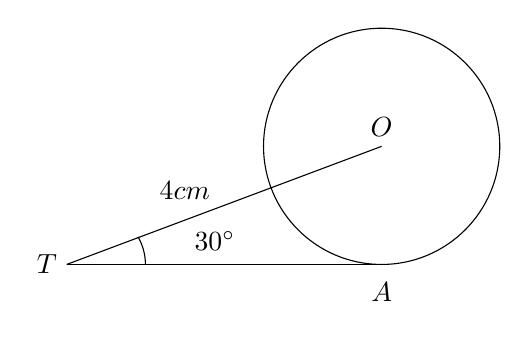
\begin{tikzpicture}
          \draw(0,0)circle(1.5cm);
          \draw(-4,-1.5)--(0,0);
          \draw(-4,-1.5)--(0,-1.5);
          \draw(-3,-1.5)arc(0:30:0.7cm);
          \node[above]at(0,0){$O$};
          \node[below]at(0,-1.6){$A$};
          \node[right]at(-2.5,-1.2){$30^{\circ}$};
          \node[left]at(-4,-1.5){$T$};
          \node[above]at(-2.5,-0.8){$4cm$};
\end{tikzpicture}
\end{flushright}

	\caption{}
	\label{fig:8}
  \end{figure}





\item In the given \figref{9},$PT$ is a tangent at $\vec{T}$ to the circle with centre $\vec{O}$.If $\angle TPO=25^{\circ}$, then $x$ is equal to:
   \begin{enumerate}
       \item 25$^{\circ}$
       \item 65$^{\circ}$  
       \item 90$^{\circ}$
       \item 115$^{\circ}$
       
   \end{enumerate}




\begin{figure}[H]
	        \centering
	        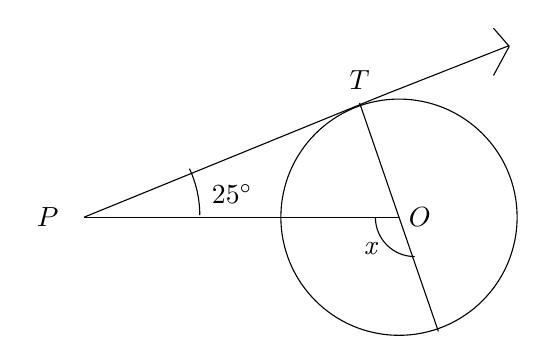
\begin{tikzpicture}
       \draw(0,0)circle(1.5cm);
       \draw(-4,0)--(0,0);
       \draw(-4,0)--(-0.2,1.55)--(1.4,2.18);
       \draw(-0.5,1.45)--(0,0)--(0.5,-1.45);
       \draw(-2.53,0.025)arc(0:25:1.4cm);
       \draw(-0.3,0)arc(180:270:0.5cm);

       \draw(1.2,2.4)--(1.4,2.17);
       \draw(1.2,1.8)--(1.4,2.17);
       
       \node[above]at(-0.5,1.5){$T$};
       \node[left]at(-4.2,0){$P$};
       \node[right]at(0,0){$O$};
       \node[left]at(-0.16,-0.4){$\textit{x}$};
       \node[right]at(-2.5,0.3){$25^{\circ}$};
   
       
\end{tikzpicture}

		\caption{}
		\label{fig:9}
\end{figure}






\item Two concentric circles are of radii 5 cm and 3 cm.Find the length of the cord of the larger circle which touches the smaller circle.

         
\end{enumerate}

\end{document}
